\documentclass[arhiv]{../izpit}
%\usepackage{fouriernc}
%\usepackage{xcolor}
%\usepackage{tikz}
\usepackage{fancyvrb}
\usepackage{enumitem}
\usepackage{tikz}
\VerbatimFootnotes{}

\begin{document}

\izpit{Programiranje I: 2.\ izpit}{9.\ februar 2021}{
  Čas reševanja je 120 minut.
  Veliko uspeha!
}

%%%%%%%%%%%%%%%%%%%%%%%%%%%%%%%%%%%%%%%%%%%%%%%%%%%%%%%%%%%%%%%%%%%%%%%
\naloga

\podnaloga
Napišite funkcijo, ki za trojico celih števil preveri ali tvorijo \emph{pitagorejsko trojico}. Trojica $(a, b, c)$ je pitagorejska, če je $a^2 + b^2$ enako $c^2$.
\begin{verbatim}
    pitagorejska_trojica : int * int * int -> bool
\end{verbatim}

\podnaloga
Napišite funkcijo, ki za celo število \verb|x| vrne celo število \verb|a|, kjer velja $\sqrt{x} \in [a, a+1)$.
\begin{verbatim}
    priblizek_korena : int -> int
\end{verbatim}

\podnaloga
Definirajte funkcijo, ki sprejme seznam celih števil in najprej \textbf{izpiše} vsa soda števila v seznamu, nato pa \textbf{izpiše} še vsa liha števila v seznamu.
\begin{verbatim}
    izpisi_soda_liha : int list -> unit
\end{verbatim}

\podnaloga
Napišite funkcijo, ki sprejme seznam elementov tipa \verb|option| in preveri, da si v seznamu izmenično sledijo konstruktorji \verb|None| in 
\verb|Some|.
\begin{verbatim}
    alternirajoci_konstruktorji : 'a option list -> bool
\end{verbatim}

\podnaloga
Funkcija \verb|najmanjsi_rezultat| naj za element \verb|x| in seznam funkcij \verb|fs| vrne \textbf{indeks} funkcije, ki ima pri argumentu \verb|x| najmanjšo vrednost izmed vseh funkcij v seznamu \verb|fs|. Ker je seznam morda prazen, naj bo rezultat tipa \verb|option|.

\textbf{Funkcija naj bo repno rekurzivna.}

\begin{verbatim}
    najmanjsi_rezultat : 'a -> ('a -> 'b) list -> int option
\end{verbatim}

%%%%%%%%%%%%%%%%%%%%%%%%%%%%%%%%%%%%%%%%%%%%%%%%%%%%%%%%%%%%%%%%%%%%%%%

\naloga

Za učinkovitejše iskanje po leksikografsko urejenih parih bomo uporabili \emph{leksikografska drevesa}, ki jih ustvarimo s pomočjo binarnih dreves.

\begin{verbatim}
    type 'a tree = Empty | Node of 'a tree * 'a * 'a tree
\end{verbatim}

Leksikografsko drevo za pare tipa \verb|'a * 'b| je binarno drevo, ki ima v
vozlišču element tipa \verb|'a| (da lahko primerjamo po prvi komponenti) in pa drevo tipa \verb|'b tree| (za primerjanje po drugi komponenti).

\begin{verbatim}
    type ('a, 'b) lexi_tree = ('a * 'b tree) tree
\end{verbatim}

Par \verb|(a, b)| se nahaja v leksikografskem drevesu, če imamo v drevesu vozlišče s parom \verb|(a, subtree)| in se \verb|b| nahaja v \verb|subtree|.

Primer drevesa za pare \verb|(3, "g")|, \verb|(3, "t")|, \verb|(7, "a")|, \verb|(10, "e")|, \verb|(10, "r")|, \verb|(10, "t")| in \verb|(10, "z")| je:

\[
  \begin{tikzpicture}[level distance=2.5cm,
    level 1/.style={sibling distance=4cm},
    level 2/.style={sibling distance=2cm}
    ]
    \node[rectangle, draw, label=left:\textbf{7}] 
        {\begin{tikzpicture}[level distance=1cm]
            \node [circle,draw] {a};
        \end{tikzpicture}}
    child {node [rectangle, draw, label=left:\textbf{3}] 
        {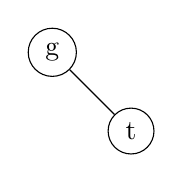
\begin{tikzpicture}[level distance=1cm, level 1/.style={sibling distance=1cm}]
            \node [circle,draw] {g}
                child { node [circle,draw, xshift=1cm] {t}};
        \end{tikzpicture}}
        }
    child {node [rectangle, draw, label=left:\textbf{4}] 
        {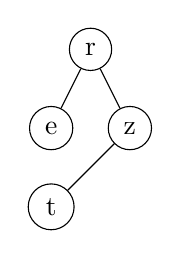
\begin{tikzpicture}[level distance=1cm, level 1/.style={sibling distance=1cm}]
            \node [circle,draw] {r}
                child { node [circle,draw] {e}}
                child { node [circle,draw] {z}
                    child {node [circle,draw, xshift=-1cm] {t}}};
        \end{tikzpicture}}
        }
    ;
  \end{tikzpicture}
\]


\podnaloga 
V OCamlu definirajte primer, ki ustreza zgornjemu leksikografskemu drevesu.

\podnaloga 
Napišite funkcijo, ki preveri ali je par prisoten v leksikografskem drevesu.

\podnaloga 
Napišite funkcijo za vstavljanje elementov v leksikografsko drevo. Če je element že v drevesu vrnite nespremenjeno drevo.

\podnaloga 
Napišite funkcijo \verb|lexi_fold|, ki sprejme funkcijo \verb|f| in začetno vrednost akumulatorja, nato pa funkcijo \verb|f| zloži preko leksikografskega drevesa. Vrstni red zlaganja je določen z leksikografsko urejenostjo.

\begin{verbatim}
    lexi_fold : ('a -> 'b -> 'c -> 'a) -> 'a -> ('b, 'c) lexi_tree -> 'a
\end{verbatim}

\podnaloga 
Definirajte funkcijo, ki vrne urejen seznam vseh elementov, ki se nahajajo v leksikografskem drevesu.


%%%%%%%%%%%%%%%%%%%%%%%%%%%%%%%%%%%%%%%%%%%%%%%%%%%%%%%%%%%%%%%%%%%%%%%

\naloga
\emph{Nalogo lahko rešujete v Pythonu ali OCamlu.}

Psička Nara po njivi preganja krokarje. Opazila je, da jo lastnik čaka na drugem koncu polja, zato hiti k njemu, pri tem pa hoče prestrašiti kar se da veliko ubogih ptičev.

Njivo predstavimo kot matriko, ki v vsakem polju vsebuje število krokarjev, ki jih pasja navihanka prežene, če teče preko tega polja.

\[
\begin{bmatrix}
2& 3& 0& 2& 9\\
8& 3& 5& 1& 2\\
1& 2& 7& 2& 0\\
4& 3& 6& 5& 5
\end{bmatrix}
\]

\podnaloga
Nara se nahaja v zgornjem levem kotu njive (polje $(0, 0)$). Ker se ji mudi k lastniku, se vztrajno premika desno. Na vsakem koraku se lahko premakne:
\begin{itemize}
\item desno
\item diagonalno desno-gor
\item diagonalno desno-dol
\end{itemize}

Pregon krokarjev zaključi na poljubnem skrajno desnem polju njive. Napišite funkcijo, ki izračuna največje število krokarjev, ki jih lahko nagajivka prežene.

\podnaloga
Funkcijo iz točke (a) prilagodite tako, da ji dodatno podate indeks vrstice, v kateri Nara začne, in indeks vrstice, v kateri Nara konča. Funkcija naj vrne seznam \textbf{vseh} optimalnih poti, kjer pot predstavimo s seznamom indeksov polj, preko katerih Nara teče.
\end{document}